\subsection{OB-26 (ZSB)}
Řízení zranitelností (vulnerability management) a záplatování (patch management), základní pojmy a proces řízení zranitelností.

\begin{itemize}
	\item proces řešení technických zranitelností jako klíč k zajištění bezpečnosti
	\item zranitelnost --- slabina v systému nebo jeho součástech
	\item technická zranitelnost --- slabina v hardware, software nebo firmware čí chyba v designu a konfiguraci systému, které umožňuje hrozbám způsobit bezpečnostní událost/incident
	\item řízení zranitelností je důležitá činnost k zabezpečení systému, který často obsahuje technické zranitelnosti (kolem 20k dokumentovaných zranitelností ročně)
\end{itemize}

\subsubsection*{Proces řízení zranitelností}
\begin{itemize}
	\item asset inventory --- identifikace součástí systému/sítě
	\item asset prioritization --- určení, v jakém pořadí/prioritě budeme součásti/zařízení/systémy řešit
	\item vulnerability assesment --- identifikace zranitelností na součástech/zařízeních/systémech, typicky se po\-uží\-va\-jí automatizované nástroje --- ohodnocení zranitelností a jejich dopadu na byznys
	\item remediation (náprava) --- začíná se od nejzávažnějších zranitelností, čím závažnější, tím rychleji se musí vyřešit a nasadit náprava
	\begin{itemize}
		\item součástí je Patch Management (PM) --- řízení záplatování
		\item kontrolují se systémy a jejich případné existující záplaty
		\item vytvoří se záplata (či se použije záplata od výrobce, pokud se jedná o cizí systém)
		\item prioritizace záplat
		\item otestování
		\item nasazení
		\item dokumentace
	\end{itemize}
	\item v případě kdy záplata neexistuje, jsou použita jiná nápravná opatření, či je systém vyřazen z provozu
	\item verification --- ověření že byla zranitelnost odstraněna
\end{itemize}

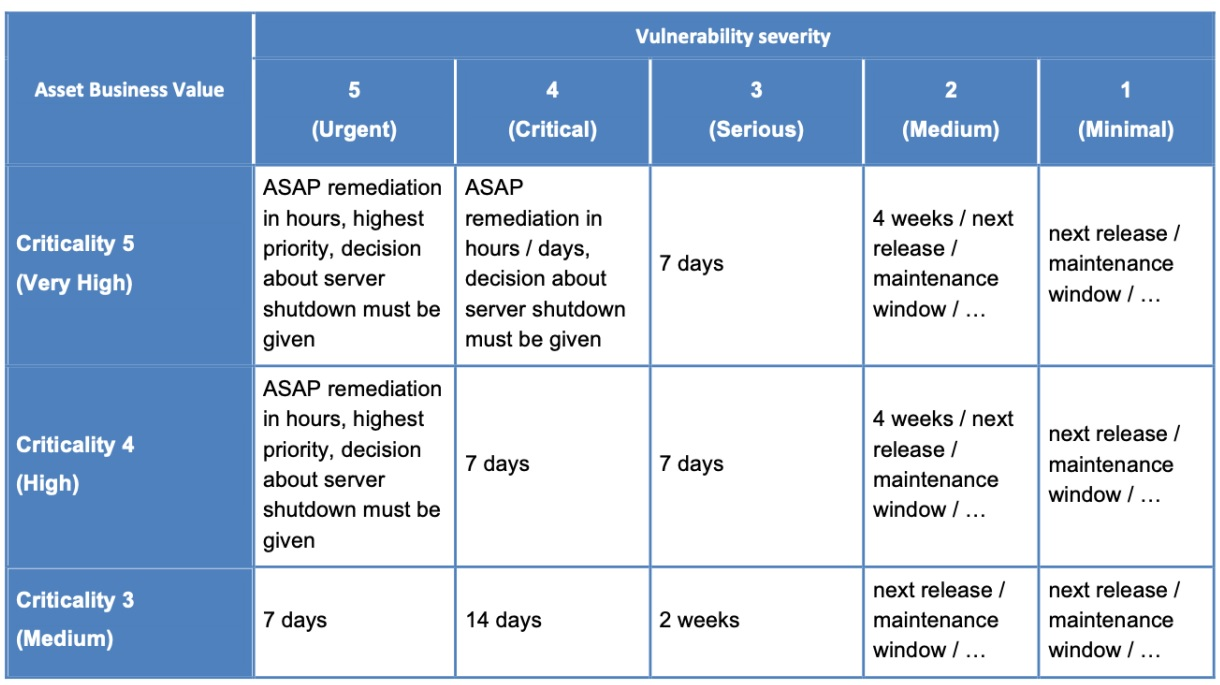
\includegraphics[width=0.9\textwidth]{img/OB-26_0.jpg}